\subsection{Options Database}
\begin{frame}[fragile]{Objects}
  % \begin{lstlisting}
  %   Mat A;
  %   PetscInt m,n,M,N;
  %   MatCreate(comm,&A);
  %   MatSetSizes(A,m,n,M,N);      /* or PETSC_DECIDE */ 
  %   MatSetOptionsPrefix(A,"foo_");
  %   MatSetFromOptions(A);
  %   /* Use A */
  %   MatView(A,PETSC_VIEWER_DRAW_WORLD);
  %   MatDestroy(A);
  % \end{lstlisting}
  \begin{minted}{c}
    Mat A;
    PetscInt m,n,M,N;
    MatCreate(comm,&A);
    MatSetSizes(A,m,n,M,N);      /* or PETSC_DECIDE */ 
    MatSetOptionsPrefix(A,"foo_");
    MatSetFromOptions(A);
    /* Use A */
    MatView(A,PETSC_VIEWER_DRAW_WORLD);
    MatDestroy(A);
  \end{minted}
  \begin{itemize}
  \item \code{Mat} is an opaque object (pointer to incomplete type)
    \oneitem{Assignment, comparison, etc, are cheap}
  \item What's up with this ``Options'' stuff?
    \begin{itemize}
    \item Allows the type to be determined at runtime: \code{-foo\_mat\_type sbaij}
    \item Inversion of Control similar to ``service locator'', \\
      related to ``dependency injection''
    \item Other options (performance and semantics) can be changed at
      runtime under \code{-foo\_mat\_}
    \end{itemize}
  \end{itemize}
\end{frame}

\begin{frame}{Basic {\kb PetscObject} Usage}

\vbox{Every object in PETSc supports a basic interface}

\begin{tabular}{|r|l|}
\hline
Function & Operation \\
\hline
{\kb Create()}               & create the object \\
{\kb Get/SetName()}          & name the object \\
{\kb Get/SetType()}          & set the implementation type \\
{\kb Get/SetOptionsPrefix()} & set the prefix for all options \\
{\kb SetFromOptions()}       & customize object from the command line \\
{\kb SetUp()}                & preform other initialization \\
{\kb View()}                 & view the object \\
{\kb Destroy()}              & cleanup object allocation \\
\hline
\end{tabular}

\vbox{Also, all objects support the {\kb -help} option.}

\end{frame}


\begin{frame}{Ways to set options}
  \begin{itemize}
  \item Command line
  \item Filename in the third argument of \code{PetscInitialize()}
  \item \code{$\sim$/.petscrc}
  \item \code{\$PWD/.petscrc}
  \item \code{\$PWD/petscrc}
  \item \code{PetscOptionsInsertFile()}
  \item \code{PetscOptionsInsertString()}
  \item \code{PETSC\_OPTIONS} environment variable
  \item command line option \code{-options\_file [file]}
  \end{itemize}
\end{frame}

\begin{frame}{Try it out}
  \shell{\small cd \$PETSC\_DIR/src/snes/examples/tutorials \&\& make ex5} \\
  \begin{itemize}
  \item \shell{./ex5 -da\_grid\_x 10 -da\_grid\_y 10 -par 6.7 \\
      -snes\_monitor -\{ksp,snes\}\_converged\_reason \\
      -snes\_view}
  \item \shell{./ex5 -da\_grid\_x 10 -da\_grid\_y 10 -par 6.7 \\
      -snes\_monitor -\{ksp,snes\}\_converged\_reason \\
      -snes\_view -mat\_view\_draw -draw\_pause 0.5}
  \item \shell{./ex5 -da\_grid\_x 10 -da\_grid\_y 10 -par 6.7 \\
      -snes\_monitor -\{ksp,snes\}\_converged\_reason \\
      -snes\_view -mat\_view\_draw -draw\_pause 0.5 \\
      -pc\_type lu -pc\_factor\_mat\_ordering\_type natural}
  \item Use \code{-help} to find other ordering types
\end{itemize}
\end{frame}

\begin{frame}[fragile]{Sample output}
\begin{Verbatim}[formatcom=\footnotesize]
  0 SNES Function norm 1.139460779565e+00 
  Linear solve converged due to CONVERGED_RTOL iterations 1
  1 SNES Function norm 4.144493702305e-02 
  Linear solve converged due to CONVERGED_RTOL iterations 1
  2 SNES Function norm 6.309075568032e-03 
  Linear solve converged due to CONVERGED_RTOL iterations 1
  3 SNES Function norm 3.359792279909e-04 
  Linear solve converged due to CONVERGED_RTOL iterations 1
  4 SNES Function norm 1.198827244256e-06 
  Linear solve converged due to CONVERGED_RTOL iterations 1
  5 SNES Function norm 1.545029314765e-11 
\end{Verbatim}
\vspace{-1em}

\includegraphics[width=0.5\textwidth]{figures/Ex5NaturalFill}
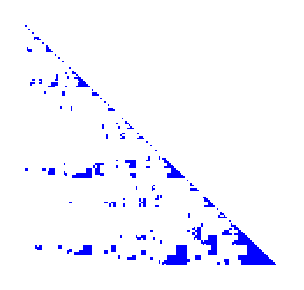
\includegraphics[width=0.5\textwidth]{figures/Ex5NDFill}
\end{frame}

\begin{frame}[fragile]{Sample output (SNES and KSP)}
\begin{Verbatim}[formatcom=\footnotesize]
SNES Object: 1 MPI processes
  type: ls
    line search variant: CUBIC
    alpha=1.000000000000e-04, maxstep=1.000000000000e+08, minlambda=1.000000000000e-12
    damping factor=1.000000000000e+00
  maximum iterations=50, maximum function evaluations=10000
  tolerances: relative=1e-08, absolute=1e-50, solution=1e-08
  total number of linear solver iterations=5
  total number of function evaluations=6
  KSP Object:   1 MPI processes
    type: gmres
      GMRES: restart=30, using Classical (unmodified) Gram-Schmidt Orthogonalization with no iterative refinement
      GMRES: happy breakdown tolerance 1e-30
    maximum iterations=10000, initial guess is zero
    tolerances:  relative=1e-05, absolute=1e-50, divergence=10000
    left preconditioning
    using PRECONDITIONED norm type for convergence test
\end{Verbatim}
\end{frame}
\begin{frame}[fragile]{Sample output (PC and Mat)}
\begin{Verbatim}[formatcom=\footnotesize]
  PC Object:   1 MPI processes
    type: lu
      LU: out-of-place factorization
      tolerance for zero pivot 2.22045e-14
      matrix ordering: nd
      factor fill ratio given 5, needed 2.95217
        Factored matrix follows:
          Matrix Object:           1 MPI processes
            type: seqaij
            rows=100, cols=100
            package used to perform factorization: petsc
            total: nonzeros=1358, allocated nonzeros=1358
            total number of mallocs used during MatSetValues calls =0
              not using I-node routines
    linear system matrix = precond matrix:
    Matrix Object:     1 MPI processes
      type: seqaij
      rows=100, cols=100
      total: nonzeros=460, allocated nonzeros=460
      total number of mallocs used during MatSetValues calls =0
        not using I-node routines
\end{Verbatim}
\end{frame}

\begin{frame}{In parallel}
  \begin{itemize}
  \item \shell{mpiexec -n 4 \\
      ./ex5 -da\_grid\_x 10 -da\_grid\_y 10 -par 6.7 \\
      -snes\_monitor -\{ksp,snes\}\_converged\_reason \\
      -snes\_view -sub\_pc\_type lu}
  \item How does the performance change as you
    \begin{itemize}
    \item vary the number of processes (up to 32 or 64)?
    \item increase the problem size?
    \item use an inexact subdomain solve?
    \item try an overlapping method: \code{-pc\_type asm -pc\_asm\_overlap 2}
    \item simulate a big machine: \code{-pc\_asm\_blocks 512}
    \item change the Krylov method: \code{-ksp\_type ibcgs}
    \item use algebraic multigrid: \code{-pc\_type hypre}
    \item use smoothed aggregation multigrid: \code{-pc\_type ml}
    \end{itemize}
  \end{itemize}
\end{frame}
